\documentclass{article}
\usepackage{graphicx} % Required for inserting images
\usepackage{amsmath}
\usepackage{amssymb}
\usepackage{indentfirst}
\usepackage{hyperref}
\usepackage{siunitx}

\title{Population-weighted meteorological zonal aggregation per administrative boundary}
\author{Tuyen Huynh}
\date{December 2024}

\begin{document}

\maketitle

\section{Problem statement}

We want to generate a single value of a weather variable for each day for each of the 24 districts in Ho Chi Minh City (HCMC), Vietnam. The problem is that weather variables are stored in a spatio-temporal raster, while districts are polygons (see \autoref{fig:district-shp}). Hence, we need to define how to aggregate weather values from raster for each district (see \autoref{fig:district-shp-intersect-raster}). Moreover, population throughout the city and within each district is not uniformly distributed (see \autoref{fig:pop-count-rast}). Since our ultimate goal is to compute risk of infection, the spatial population distribution needs to be taken into account while performing weather raster aggregation, i.e. give more weight to weather values where people actually live in a district.

\begin{figure}
    \centering
    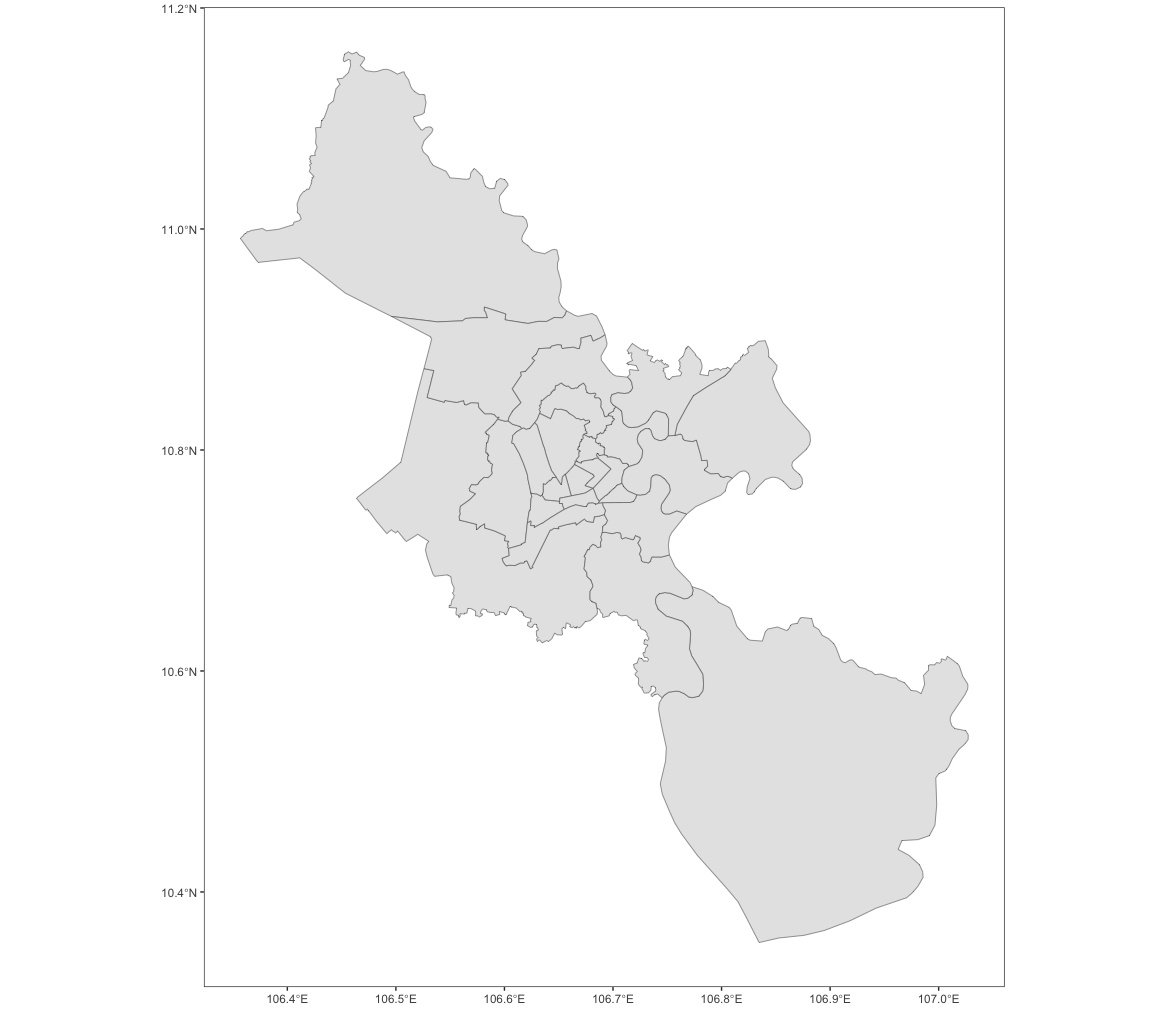
\includegraphics[width=0.8\linewidth]{district_shp.png}
    \caption{Map of administrative boundaries of 24 districts in HCMC, Vietnam}
    \label{fig:district-shp}
\end{figure}

\begin{figure}
    \centering
    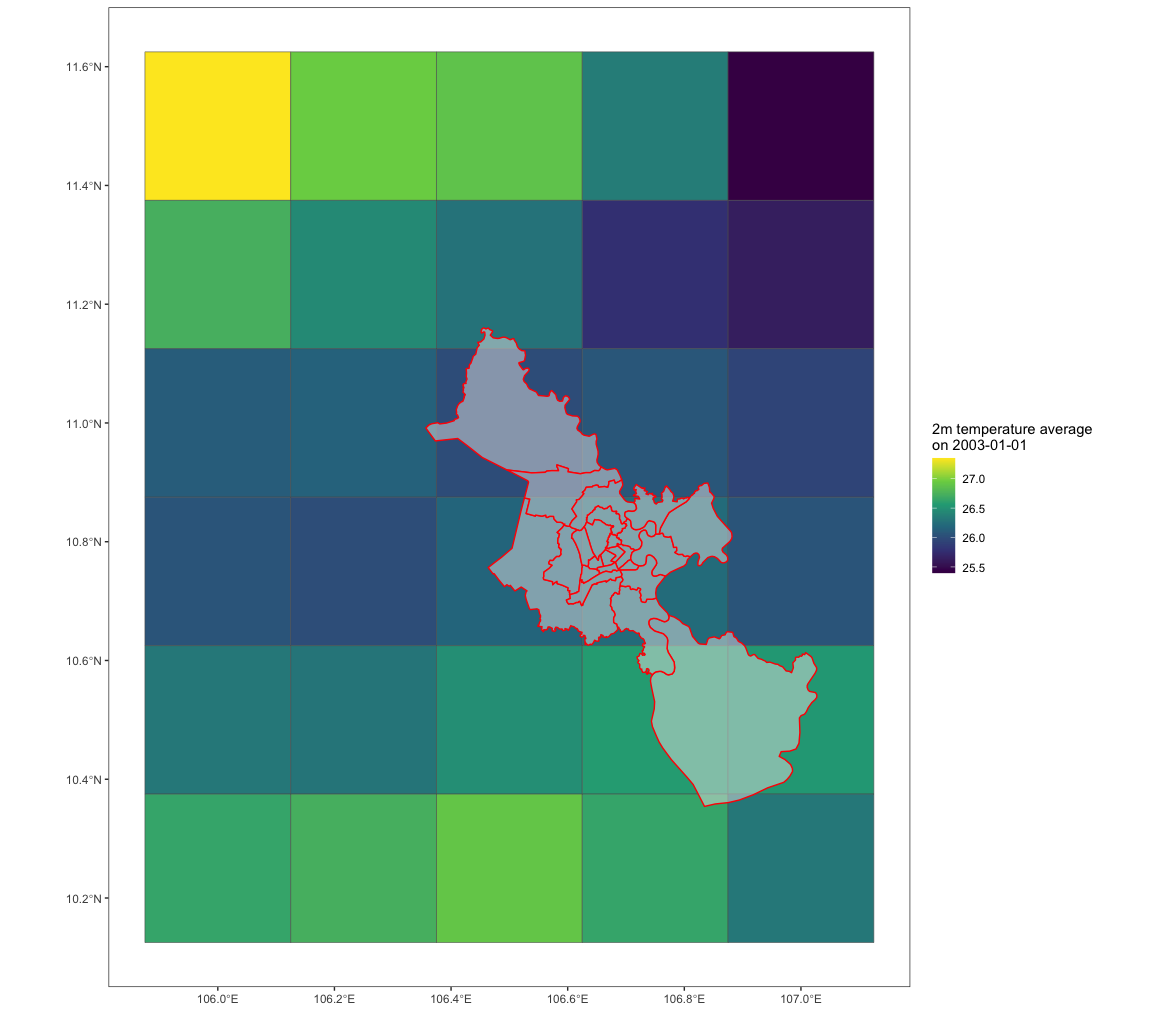
\includegraphics[width=0.8\linewidth]{district_shp_w_raster_color.png}
    \caption{Weather raster cells overlayed with HCMC district boundaries. Colored by average 2m temperature on 2003-01-01.}
    \label{fig:district-shp-intersect-raster}
\end{figure}

\begin{figure}
    \centering
    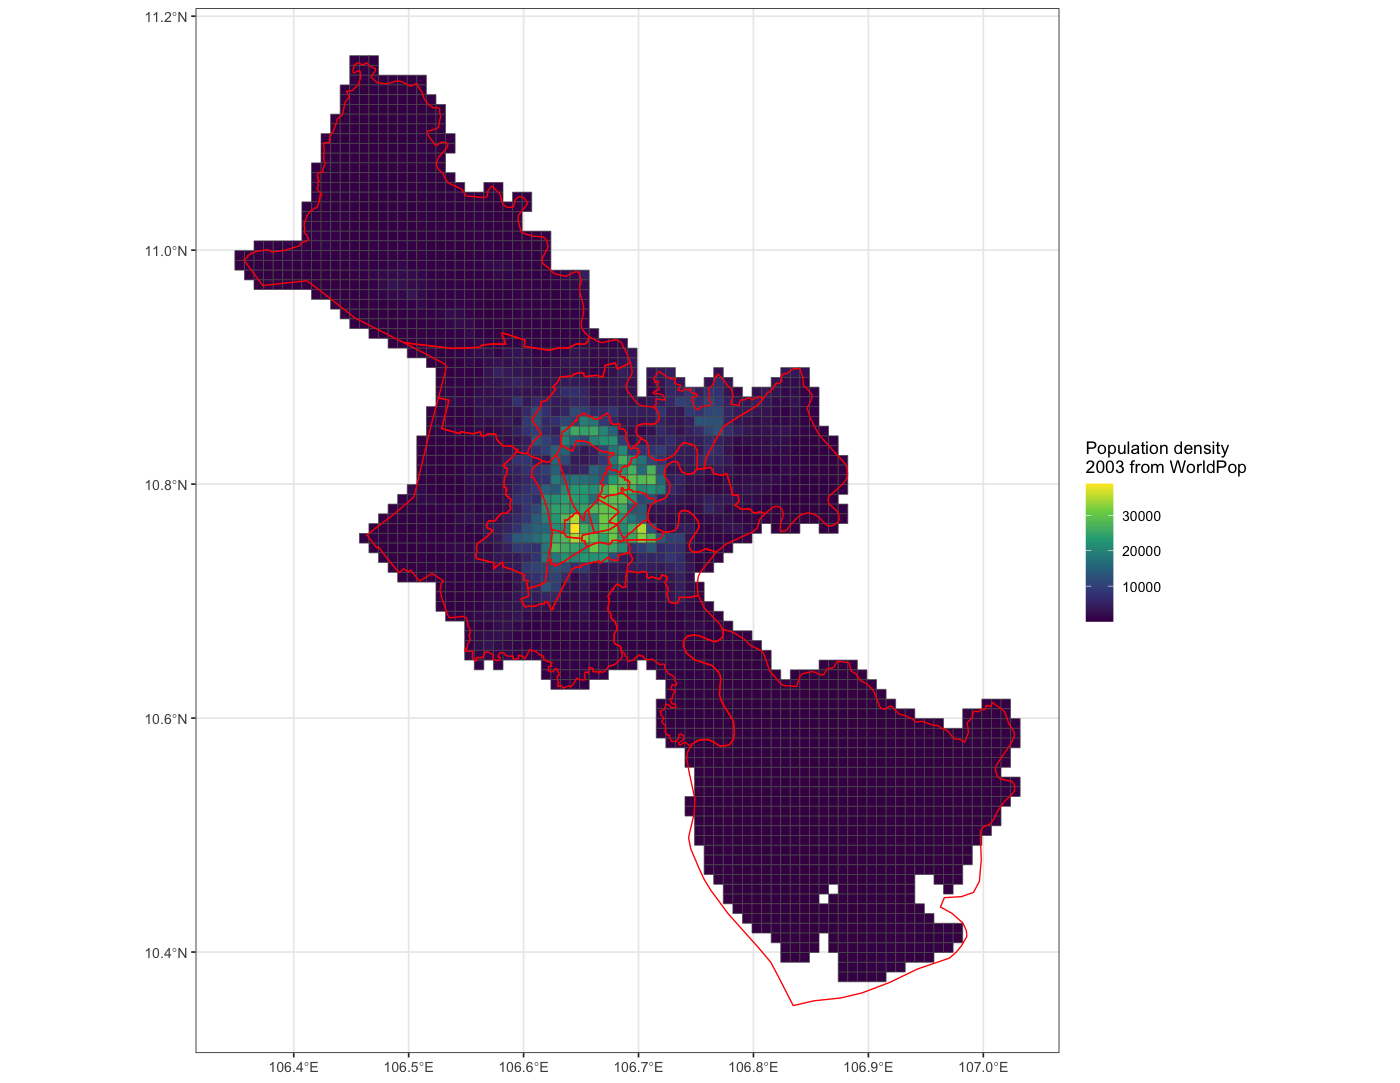
\includegraphics[width=0.8\linewidth]{pop_count_rast.png}
    \caption{2003 population counts estimation raster for HCMC from WorldPop. Red outline shows the administrative boundaries of distrcts}
    \label{fig:pop-count-rast}
\end{figure}

\section{Definitions}

\subsection{What a polygon is}

A polygon is an ordered set of points on a 2-dimensional Cartesian coordinate system that produces a closed shape, i.e. where the first and last points are the same. A point is called a \textbf{vertex}. Each vertex has a pair of coordinates $(x, y)$. The line drawn between 2 vertices is called an \textbf{edge}. The edges of a polygon together define its \textbf{boundary}. A polygon can also have an associated value. In this context, each district is a polygon, based on its administrative boundaries provided by GADM (https://gadm.org/index.html).

\subsection{What a raster is}

A raster has a spatial component and a temporal component. Spatially, a raster $R$ is a $(n_\text{rows} \times n_\text{cols})$ matrix of cells $R_i$.

\begin{equation*}
    R = \{R_{i}\}, i \in [1, n_\text{cells}]
\end{equation*}

where $n_\text{cells} = n_\text{rows} \cdot n_\text{cols}$ is the number of cells in the raster. A raster is typically overlayed over a geographical region, for example, \autoref{fig:district-shp-intersect-raster} is a weather raster overlayed over the administrative boundary of HCMC. Temporally, a raster can be viewed as a sequence of rasters over 

\subsection{Geometry and associated value of a polygon} \label{sect:poly-props}

A polygon contains an ordered set of coordinates of its vertices, i.e. its geometry. In addition, it can also have an associated value. Given each raster cell $R_i$ is also a polygon itself (more specifically, a square), they can also have an associated value. For example, in a weather raster, each cell would store values of temperature and precipitation; in a population count raster, each cell would store a value of population count. 

We then define $\gamma$ and $\nu$ as the functions that extracts the geometry and the associated value of a polygon, respectively. We also define $\operatorname{area}$ as the function that calculates the surface area of a geometry.

\section{The intersection of two polygons}

2 polygons are intersecting if at least a pair of edges from each are intersecting or all the vertices of one are within the boundary of the other one. If 2 polygons are intersecting, they share some surface area. Testing whether 2 polygons intersect is implemented by the \verb|st_intersects()| function of the \verb|sf| package in the R programming environment. 

The intersection $P_i \cap P_j$ of 2 polygons $P_i$ and $P_j$ produces a new polygon made up of their shared surface area. This operation is commutative. There are 3 scenarios when intersecting: (i) If $P_i$ is within $P_j$, the resulting polygon from the intersection would be identical to $P_i$; (ii) If $P_i$ and $P_j$ do not intersect, the result will be an empty set $\emptyset$; (iii) If prior scenarios do not apply, then the 2 polygons are \textbf{partially intersected}. The intersection of 2 polygon is implemented by the \verb|st_intersection()| function also from \verb|sf|. 

Given a raster $R$ and district polygon $D$, the intersection between them is the intersection of each raster cell $R_i$ and $D$, producing a new set of polygons defined as:

\begin{equation*}
    P = \{ \gamma(R_i) \cap D \}
\end{equation*}

As described above, the new polygon $P_i$ can be: (i) exactly same as $R_i$, (ii) an empty set $\emptyset$, or (iii) made up of shared surface area between $R_i$ and $D$. This is visualised in \autoref{fig:intersect-proc} panel (a), using a population count raster where $\Delta = 1\si{km}$.

\subsection{Dealing with partial intersection}
Given that some new $P_i$ will have a smaller surface area than its original $\gamma(R_i)$ (scenario (iii)), $\nu(P_i)$ is calculated by weighting the ratio of new and original surface area:

\begin{equation} \label{eq:recalc-intersect}
    \nu(P_i) \equiv \nu(R_i)\frac{\operatorname{area}(\gamma(P_i))}{\operatorname{area}(\gamma(R_i))}
\end{equation}

% $\nu(P_i) \equiv \nu(R_i)\frac{\gamma(R_i \cap D)}{\gamma(R_i)}$

This is visualised in \autoref{fig:intersect-proc} panel (b).

\begin{figure}
    \centering
    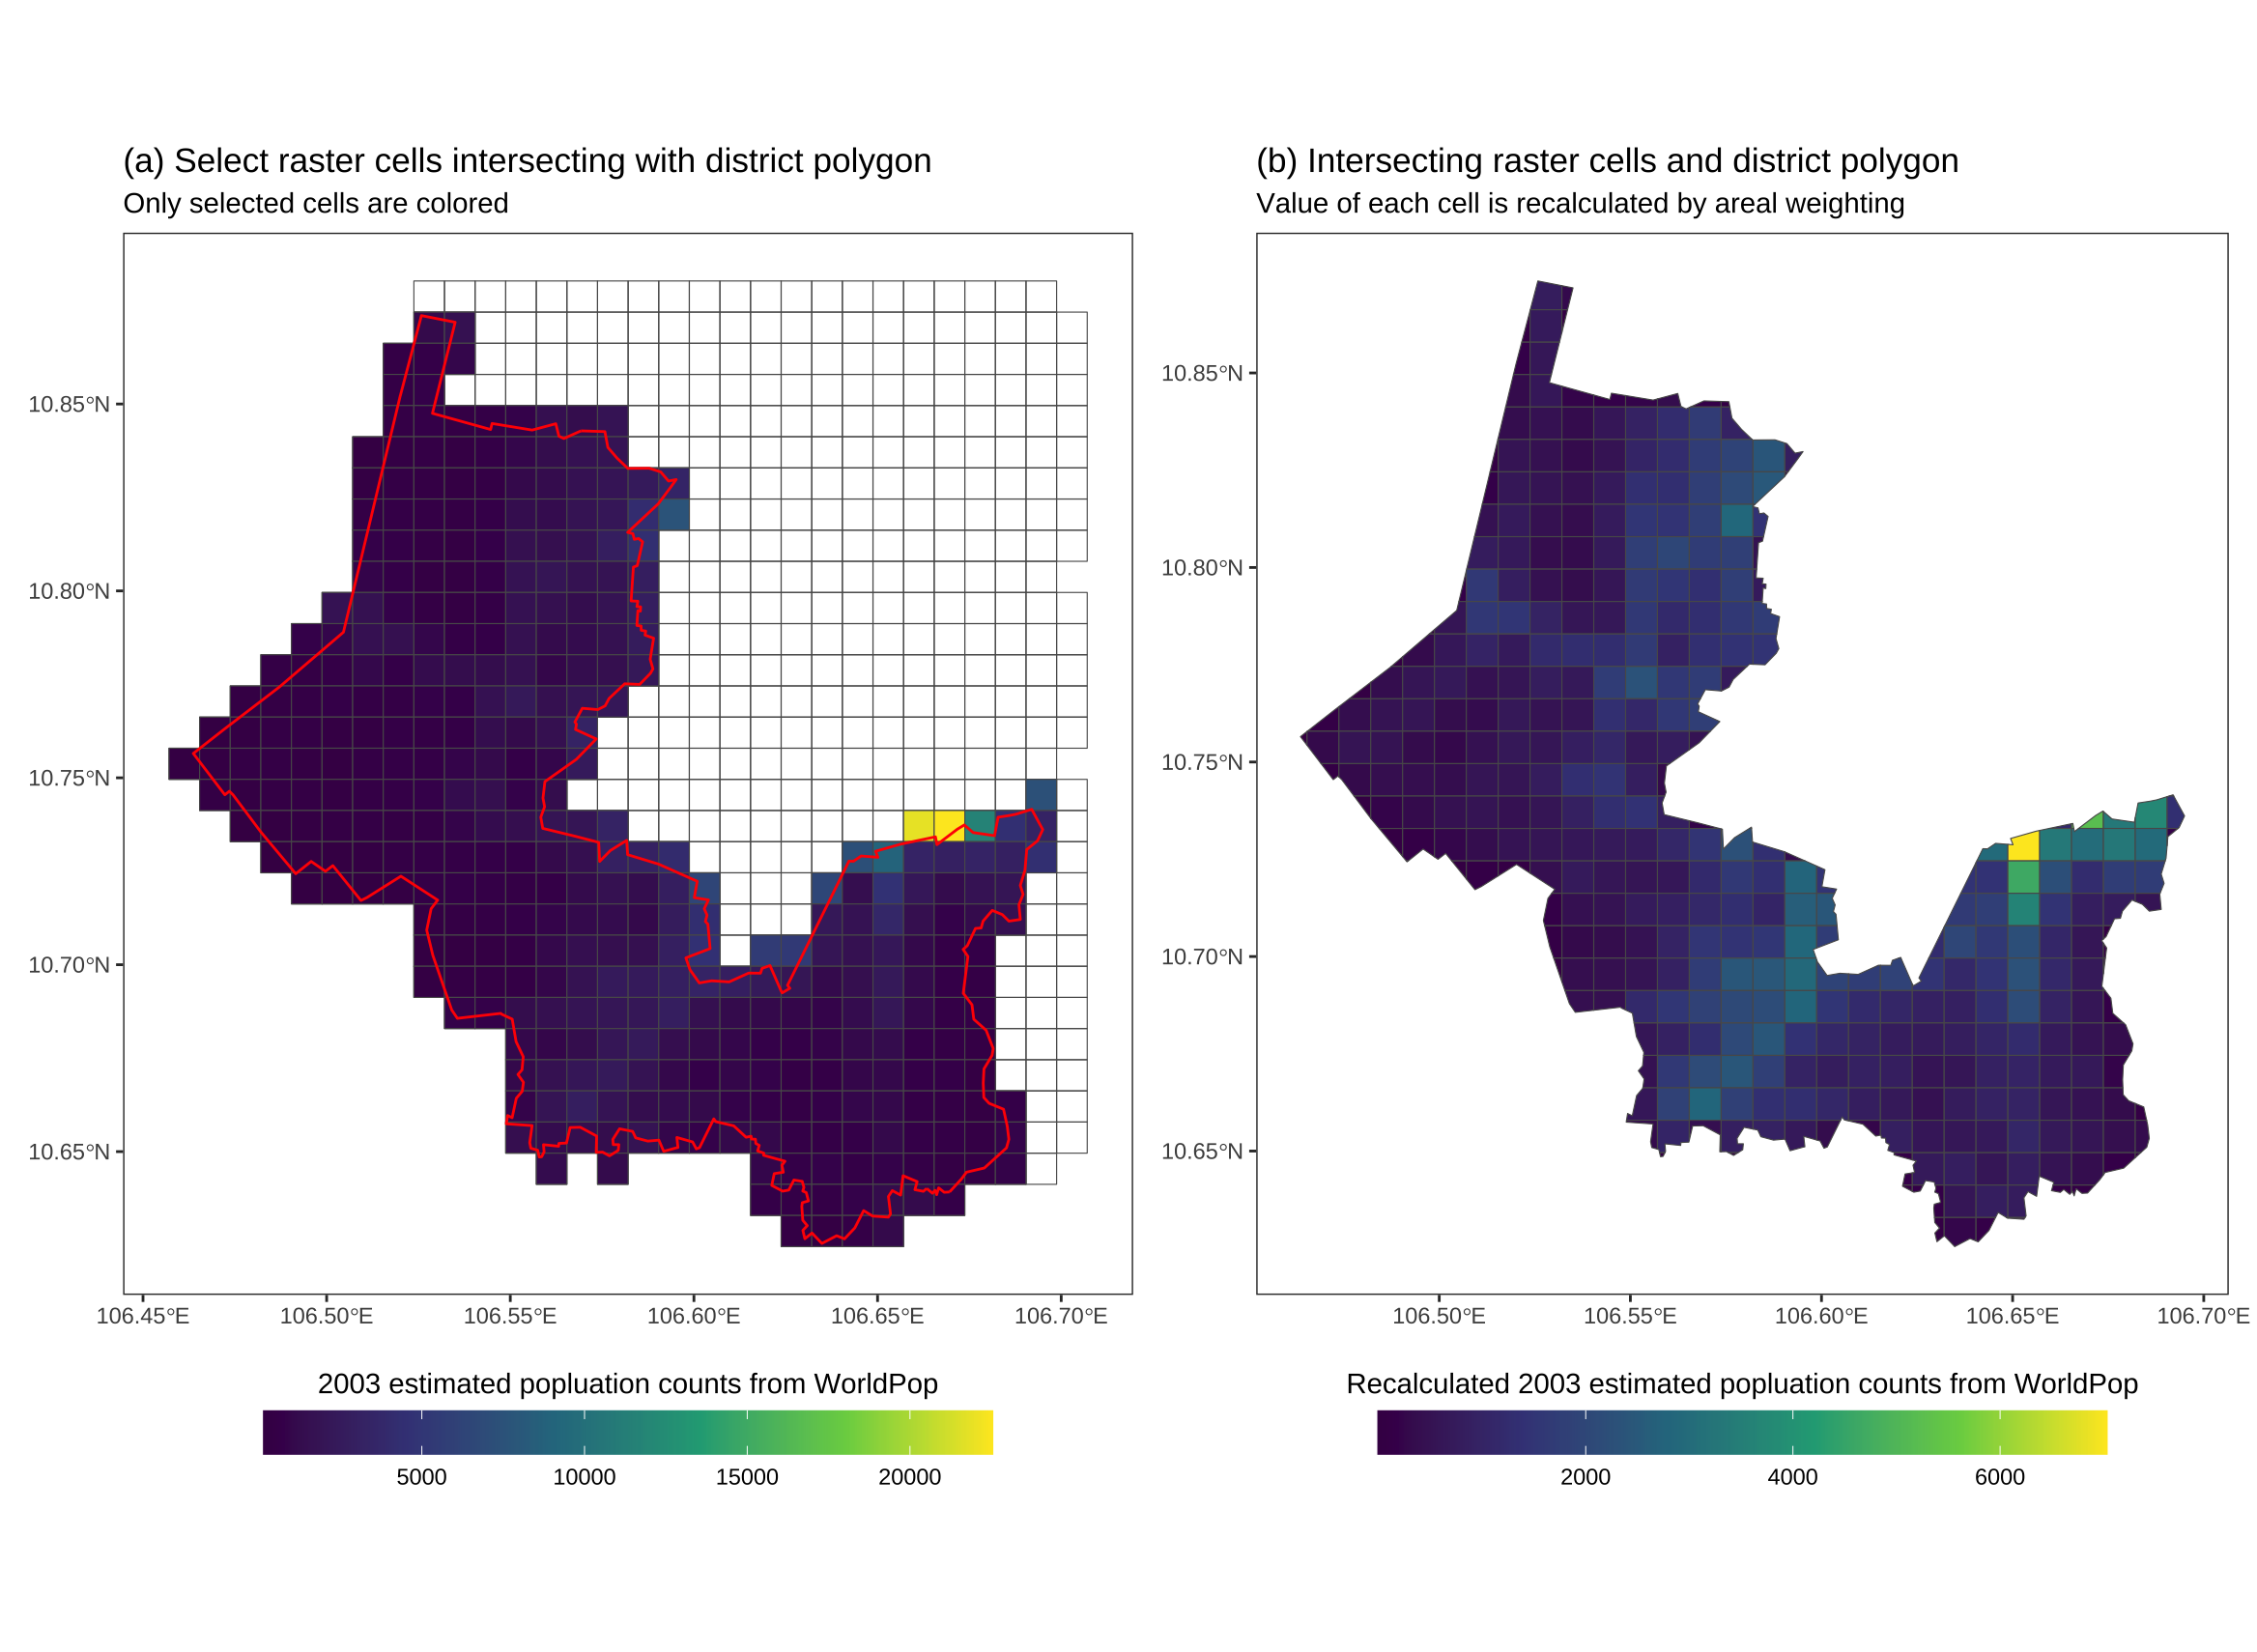
\includegraphics[width=1\linewidth]{intersection_process.png}
    \caption{Process of intersecting a raster $R$ and a district polygon $D$. All raster cells $R_i$ act as a geometry using $\gamma(R_i)$ as defined in \ref{sect:poly-props}. (a) shows how $R_i$ are considered intersecting with district by having at least one crossing edge-pair or within $D$. (b) shows how intersecting 2 polygons creates a new polygons. The colored cells are recalculated as defined in \autoref{eq:recalc-intersect}.}
    \label{fig:intersect-proc}
\end{figure}

% , effectively creating a set of indices $i \in \{R \cap G\}$, where $R_i$ is the subset of raster cells that \textbf{intersects} the geometry and are \textbf{covered by} the geometry. 

\section{District zonal aggregation}

For each day $t$, given weather raster $R$, district polygon $D$, and population count raster $P$, the district zonal aggregation is defined as:

\begin{equation*}
    \nu(D(t)) = \sum_{R_i \in R}{ \nu(R_i(t))
            \frac
            { \sum_{Q_i \in \{\gamma(R_i) \cap \{D \cap P\}\}} \nu(Q_i)}
            { \sum_{P_i \in \{D \cap P\}} \nu(P_i)}
        }
\end{equation*}


where

\begin{itemize}
    \item $Q_i$ is a polygon produced by intersecting 3 polygons $R_i$, $D$ and $P$
    \item $\nu(Q_i)$ and $\nu(P_i)$ are the weighted value using \autoref{eq:recalc-intersect}
\end{itemize}

See \autoref{fig:aggregation} for a visual presentation of this aggregation method.

\begin{figure}
    \centering
    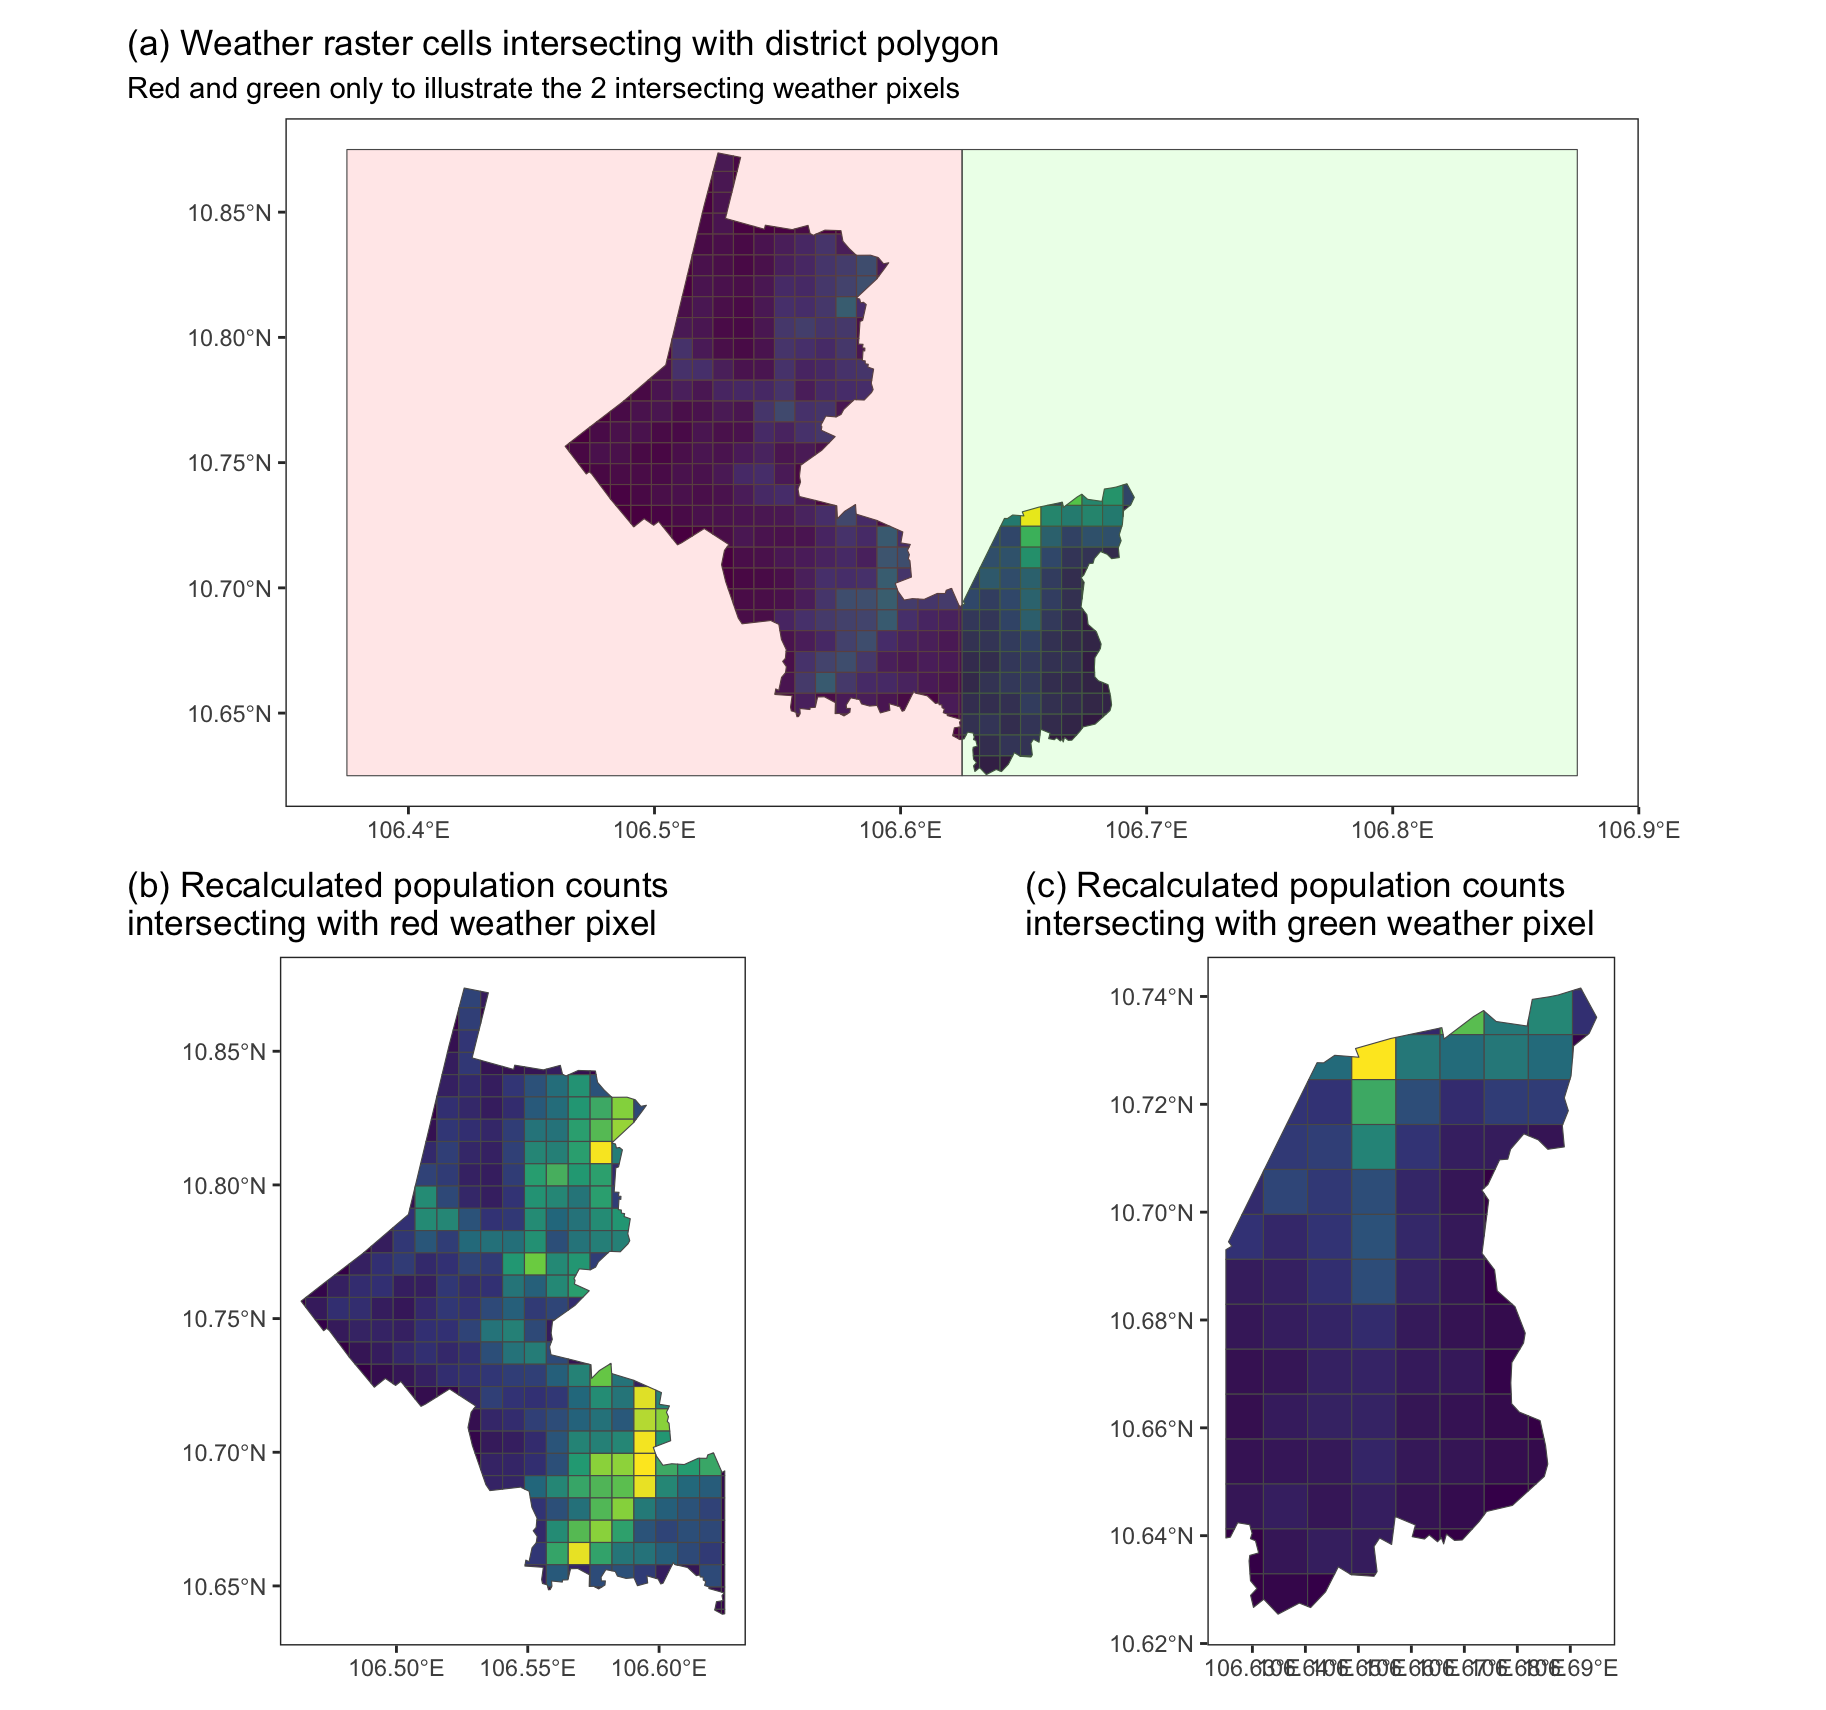
\includegraphics[width=1\linewidth]{aggregation.png}
    \caption{Visual presentation of the aggregation method. Using Bình Chánh district, 2003 population counts and first time point in the intersecting weather raster (with alpha = 0.1). Red and green hues specify the different intersections of population counts and weather raster cells that will be used as weights for each weather raster cell.}
    \label{fig:aggregation}
\end{figure}

\end{document}
